%-------- DOTEX main file--------------------
%-----------------------------------iam-tom-2012
\documentclass
[
a4paper,
german,
oneside,
openright,                    % Kap.beginn immer rechts! (fkt. nur bei report, nicht bei article)
12pt                          % ersatzweise 12pt, wenn mehr Seiten entstehen sollen
]
{report}

%% Packages
\usepackage{cite}
\usepackage{graphicx}
\usepackage{amsmath}
\usepackage{amssymb}
\usepackage{color}
\usepackage{tikz}
\usetikzlibrary{shapes,snakes,positioning,arrows,shadows,backgrounds}
\usepackage{caption}
\usepackage{color}
\usepackage{hyperref}
\usepackage{listings}
\synctex=1
\usepackage[utf8]{inputenc}
\usepackage{subfigure}
%%\usepackage{showframe}
\usepackage{pdfpages}
\usepackage{multicol}

%% Path settings
\graphicspath{{../img/}}

\sloppy


%% tikz settings---------------------------------------------------
\newif\iffinal % introduce a switch for draft vs. final document
%\finaltrue % use this to compile the final document

% [more preamble that in my case also uses \iffinal for other stuff]

\usepackage{tikz}
\pgfrealjobname{thesisII} % <-- NOTE: this needs to be the real document's basename
                        %     (else you'll only get an empty output file)
\iffinal
  \newcommand{\inputTikZ}[1]{%
    \input{#1.tikz}%
  }
\else
  \newcommand{\inputTikZ}[1]{%
    \beginpgfgraphicnamed{#1-external}%
    \input{#1.tikz}%
    \endpgfgraphicnamed%
  }
\fi
%% -------------------------------------------------------------------------


\begin{document}
%-------- DOTEX config file--------------------
%-----------------------------------iam-tom-2012

%% renewed commands
%%--------------------------------

%\renewcommand{\labelitemi}{-}


%% new commands
%%--------------------------------

%\newcommand{}{}
\newcommand{\idea}{\textit{\textbf{IDEA:}}\textit}
\newcommand{\lid}{\texttt{\textbf{Literature ID:}}\texttt}
\newcommand{\src}{\texttt{\textbf{}}}
\newcommand{\now}{\textbf{\today}}

% TODO IN red
\newcommand{\todo}[1]{\textcolor{red}{\textbf{TODO:} \emph{#1}}}

%% commands

\newcommand{\img}{{I}}


%CODE SNIPPETS
%%--------------------------------
%this code auto-regenerates pdf+latex from svg
\newcommand{\executeiffilenewer}[3]{%
\ifnum\pdfstrcmp{\pdffilemoddate{#1}}%
{\pdffilemoddate{#2}}>0%
{\immediate\write18{#3}}\fi%
}
\newcommand{\includesvg}[1]{%
\executeiffilenewer{#1.svg}{#1.pdf}%
{inkscape -z -D --file=#1.svg %
--export-pdf=#1.pdf --export-latex}%
\input{#1.pdf_tex}%
}




% sizhe and margin settings %
\setlength{\unitlength}{1cm}
\setlength{\oddsidemargin}{0.3cm}
\setlength{\evensidemargin}{0.3cm}
\setlength{\textwidth}{15.5cm}
\setlength{\topmargin}{-1.2cm}
\setlength{\textheight}{23cm}
\columnsep 0.5cm
%





%---chapters
      %% TEMP
      \pagestyle{plain}
      \pagenumbering{arabic}
      \setcounter{page}{3}
      \tableofcontents
      \cleardoublepage

      \listoffigures
      \protect \addcontentsline{toc}{chapter}{Abbildungsverzeichnis}
      \cleardoublepage


      \listoftables
      \protect \addcontentsline{toc}{chapter}{Tabellenverzeichnis}
      \cleardoublepage


      %\listofalgorithms
      %\protect \addcontentsline{toc}{chapter}{Algorithmenverzeichnis}
      %\cleardoublepage

      \chapter{Introduction}
\subsection{abstract}
The acceptance of service robots comes along with the ability to adapt to user specific preferences. This requires that a robot can determine the identity of the user. As for humans, robust user recognition is based on the identification of the face. However, despite the plethora of published work on face recognition that is robust against real world noise such a illumination, head alignment or facial expressions there is no robust off-the-shelf non-commercial software available to be used in typical robotics applications. Hence, this paper introduces a ready-to-use open-source ROS package providing a face detection and identification system that is comprising novel and state-of-the-art solutions to various aspects of face recognition while utilizing modern RGB-D sensors. This work demonstrates a solution for face recognition in robotic settings that is robust against varying illumination, gaze directions of the head, and facial expressions while operating with online performance. The paper provides a thorough evaluation of the face recognition system based on standard database tests and on real world scenarios regarding these criteria.


%%%%%%%%%%%%%%%%%%%%%%%%%%%%%%%%%%%%%%%%%%%%%%%%%%%%%%%%%%%%%%%%%%%%%%%%%%%%%%%%
\section{Introduction}
%- 1 Paragraph general introduction to robotics, face recognition, applications
%- 1 Paragraph concrete problem and subproblems tackled in the paper
%- we need a reference to our covergirl image somewhere in these paragraphs

With service robots becoming more and more capable of doing useful work in households appropriate user interaction becomes increasingly important. For example, in the EU-funded project Accompany we are researching how a multifunctional service robot like Care-O-bot 3 may assist elderly persons with their daily activities, like transporting items, delivery tasks, reminder functions, or grasping objects from a shelf. Such services and the interaction with the user therein are highly user specific and the robot is required to interact with multiple kinds of users in the respective ways. Hence, the identification of individual users is a crucial precondition to successful interaction.

Despite this apparent need for accurate user identification in applications for service robots there are, besides many commercial solutions, only few open-source systems available. The most prominent examples are libface \cite{jironkin2010} and the ROS stack people \cite{pantofaru2010}, which both use the Viola-Jones classifier \cite{Viola01} for face detection and Eigenfaces \cite{Turk1991} for recognition, as well as OpenCV \cite{bradski2008} itself which has been enhanced by several modern recognition algorithms recently. However, although there is a large body of research dedicated to person recognition under difficult circumstances such as varying illumination, head pose, or facial expressions, robotics could not benefit from a ready-to-use solution so far which covers all the challenges occurring in real operation. Hence, the motivation for this work was to develop a complete person identification pipeline that exploits the benefits of RGB-D streams from inexpensive RGB-D cameras and that is insensitive to typical real-world influences such as illumination, head pose, and facial expressions, while maintaining online performance for usage with real robots. Moreover, the system should be able to safely distinguish at least 30 people, detect unknown people as being new, and unknown subjects should be easily and quickly added to the database without any fancy requirements regarding the recording settings for the sample face images.

%- OpenCV provides some algorithms for detection and recognition
%- libface - uses OpenCV detection and implements Eigenfaces
%- people stack

%motivation:
%- ready-to-use person identification pipeline
%- uses RGB-D image streams
%- insensitive to typical real-world influences as illumination, head pose, facial expressions
%- real-time performance
%- quickly trainable in any situation (no fixed recording procedure or defined lighting necessary, few training images), fast integration of new training data to recognition module
%- possibility to detect unknown people as being new
%- safely distinguishing numbers up to 30 people

\begin{figure}[t]
	\begin{center}
		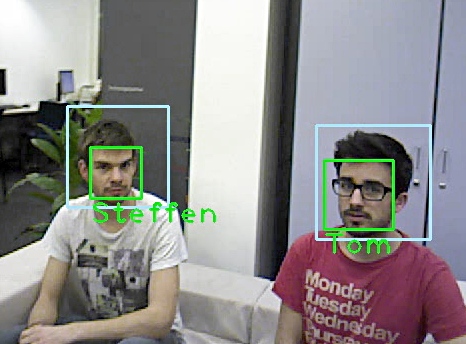
\includegraphics[width=0.76\columnwidth]{title_image.png}
	\end{center}
	\caption{Head detection (blue frame), face detection (green frame) and recognition of identity in real world service robotics applications.} \vspace{-2mm}
	\label{fig:covergirl}
\end{figure}

This paper introduces a person identification system that combines face detection based on our previous work \cite{Fischer2010}, modern preprocessing procedures and face recognition based on Fisherfaces \cite{Belhumeur1997} as well as a tracking system for continuous and robust identification of persons in RGB-D image streams. The whole system fulfills all of the mentioned requirements making it ready for the use with a real service robot. The main contributions of this work are:
\begin{enumerate}
	\item A ready-to-use open-source ROS package\footnote{the software is available as \texttt{cob\_people\_perception} stack at \url{http://www.ros.org/wiki/cob_people_perception}} providing a complete face detection and identification system that is well-suited for application in robotics domains.
	\item A combination of novel and state-of-the-art methods for RGB-D face recognition selected on the basis of a thorough literature review.
	\item A comprehensive evaluation of the face recognition system regarding the imposed criteria.
\end{enumerate}
%Highlight that our experiments prove that our implementation fulfills all these requirements achieving high recognition rates under the considered perturbations using always a small and not diverse set of training images for all tests.
%This paper discusses our follow-up work to \cite{Fischer2010} where the face detection system has been described in detail. 

The remainder of this paper is structured as follows. After a discussion of relevant work in Sec. \ref{sec:relatedwork} the utilized algorithms are explained in Sec. \ref{sec:methods}. Following the face recognition system is evaluated in Sec. \ref{sec:evaluation} with regard to accuracy and robustness aspects. The paper concludes with a summary and an outlook for following research in Sec. \ref{sec:conclusions}.

      \cleardoublepage

      \chapter{State of the art}
\label{chap:relwork}
\section{Face Detection}
\label{chap:relwork:sec:detection}
As this paper describes a complete face recognition system, the literature review covers the detection and the recognition of faces.
Face detection is the search for face regions in color images or 3d data.
The most famous face detection algorithm is the Viola-Jones detector \cite{Viola01} which constructs a rejection cascade built on Haar features.
It has been the top performing face detection method for a long time and has not been beaten until Jain and Learned-Miller \cite{jain2011} introduced an online improvement procedure for the Viola-Jones classifier.
Even better face detection results have been reported on the FDDB database \cite{jain2010} by Li et al. \cite{li2011} who construct a similarly boosted cascade on SURF features retaining a comparable computational effort.
Face recognition on 3d data has also become increasingly important.
The work of Jasek et al. \cite{Jasek2012} is one example that uses local curvature features for face detection.
Further relevant literature can be found in their publication.
Fischer et al. \cite{Fischer2010} introduced a combined system that applies the Viola-Jones classifier to depth images for head detection and to color images for face detection obtaining very good results.
Because of this and fast computation time %, that could be confirmed in our experiments,
we decided to employ this combined detector in the current work.

\section{Face Recognition}
\label{chap:relwork:sec:recognition}
Regarding face recognition, there are many well-performing algorithms available today which target at significantly different applications, invariance properties, and computational demands.
Some of the most influential approaches are projection methods \cite{Turk1991,Belhumeur1997,Naseem2010,Yan07,Yang2002,Zhang2010}, local pattern-based methods \cite{Ahonen2006, Tan2010}, generative models \cite{Georghiades01, Lee05}, sparse representations \cite{Wagner2012}, and face modeling via Hidden Markov Models \cite{Samaria1994}.

\subsection{Projection methods}
\label{chap:relwork:sec:recognition:subsec:projection}
Projection methods generally consider the pixel image as a vector in a high-dimensional space and project it into some low-dimensional space, often called face space, which is better suited for classification.
Many different projections have been proposed including famous examples like Eigenfaces \cite{Turk1991}, where the basis of the face space is spanned by eigenvectors obtained from a PCA analysis of the training images, and Fisherfaces \cite{Belhumeur1997}, where the projection bases on Fisher's Linear Discriminant and is computed to be nearly orthogonal to intra-class scatter to minimize intra-class variance while maximizing inter-class variance.
Further projection methods construct linear subspaces for each person based on the original gallery images and measure the distance of query faces to these spaces \cite{Naseem2010}, enhance the projection by kernel methods to model higher-order pixel dependencies \cite{Yang2002}, or refine the Fisherfaces approach with more intricate target subspaces \cite{Yan07, Zhang2010}.
All projection methods are characterized by a low computational complexity and all modern variants and Fisherfaces attain high recognition rates on standard databases.

\subsection{Sparse representation}
\label{chap:relwork:sec:recognition:subsec:sparse}
Similar to the approach of Naseem et al. \cite{Naseem2010} the sparse representation of Wagner et al. \cite{Wagner2012} encodes faces as linear combination of a set of gallery images, however, with the difference that the vector of coefficients and the vector of pixel corrections are optimized with an $L_1$ norm simultaneously to achieve a sparse representation.
The authors implement a preceding alignment optimization since the method relies heavily on well-aligned images.
Although providing very good recognition results this approach is not well-suited for robotics applications because of a computation time of several seconds induced by the two optimizations and the need for diverse training images.
Local pattern-based methods construct spatially constrained statistics over dense local image features and accumulate these statistics to a vector describing a face.
Ahonen et al. \cite{Ahonen2006} compute histograms over local binary patterns (LBP) in several image regions and attach the histograms to a feature vector that is matched with a $\chi^2$ measure against the gallery.
Tan and Triggs \cite{Tan2010} expand this idea to local ternary patterns and reduce the length of the high-dimensional feature vectors with General Tensor Discriminant Analysis.
Local pattern-based algorithms are counted to the top-performing face recognition methods and are usually fast to compute.

\subsection{Generative methods}
\label{chap:relwork:sec:recognition:subsec:generative}
In contrast to the discriminative approaches discussed so far, generative methods base upon the illumination cone model \cite{Basri2003} which proves that many kinds of illumination may be described by a 9-dimensional subspace.
Georghiades et al. \cite{Georghiades01} estimate the true 3d shape of a face from a set of frontal face images with variable lighting and render new poses synthetically to improve recognition performance w.r.t. head pose by computing further illumination cones for all possible alignments.
In a similar approach Lee et al. \cite{Lee05} model the appearance of arbitrarily illuminated faces by a set of 5-9 images taken with specified locations of a point light source. 
Although such generative methods do also achieve good recognition results they are not well-suited for practical usage due to the necessity for defined or various illumination conditions for training data recording.
Consequently, only projection-based and local pattern-based methods are adequate for application in robotics and hence tested within our recognition framework.
Both approaches suffer from influences like variable lighting and head pose. 

\section{Preprocessing}
\subsection{Illumination correction}
Chen et al. \cite{chen06} divide illumination correction methods into three categories: (i) modeling of the illumination cone as discussed above, (ii) extraction of invariant features, and (iii) preprocessing.
Illumination invariant features are considered edge maps, derivatives of the gray-level image, images filtered with 2D Gabor-like functions \cite{Adini1997}, and to some extent LBPs \cite{Ahonen2006}.
Preprocessing includes histogram equalization, logarithmic transform \cite{liu02}, gamma correction \cite{Goel11}, discarding the low-frequency Discrete Cosine Transform coefficients \cite{chen06}, Difference of Gaussians filtering, and contrast equalization \cite{Tan2010}.
We implemented several preprocessing methods since they can be combined with many recognition algorithms and they are computed cheaply.

\subsection{Head pose correction}
Similarly, there are many solutions to head alignment like modeling multiple orientations with the training data \cite{Georghiades01, pentland1994} or face plane estimation from local features like eyes and nose that are found in the depth image \cite{Gurbuz12, Jasek2012} or in the color image \cite{beymer1994}.
None of the discussed methods actively strives to model different facial expressions but local methods and Fisherfaces actively construct representations for filtering out such kinds of intra-class variance.


      \cleardoublepage

      \chapter{Methods}
\label{chap:methods}
The person recognition system provides algorithms for all necessary steps to detect and identify people in RGB-D data streams.
A sketch of the involved processing stages is displayed in Fig. \ref{fig:scheme}.
We first detect the location of faces in the current view using a depth image-based head detector and a color image-based face detector (Sec. \ref{sec:methods:subsec:detection}).
The detected faces are then analyzed by the face identification module which determines the names of captured persons while taking care of real world influences such as different lighting or varying face orientation (Sec. \ref{sec:methods:subsec:identification} to \ref{ssec:IdentificationUnknown}).
Finally, Sec. \ref{sec:methods:subsec:tracking} discusses the detection tracker, which ensures that persons detected in previous images can be matched to the current results while filtering out spurious false identifications.

\begin{figure}[tb]
	\begin{center}
		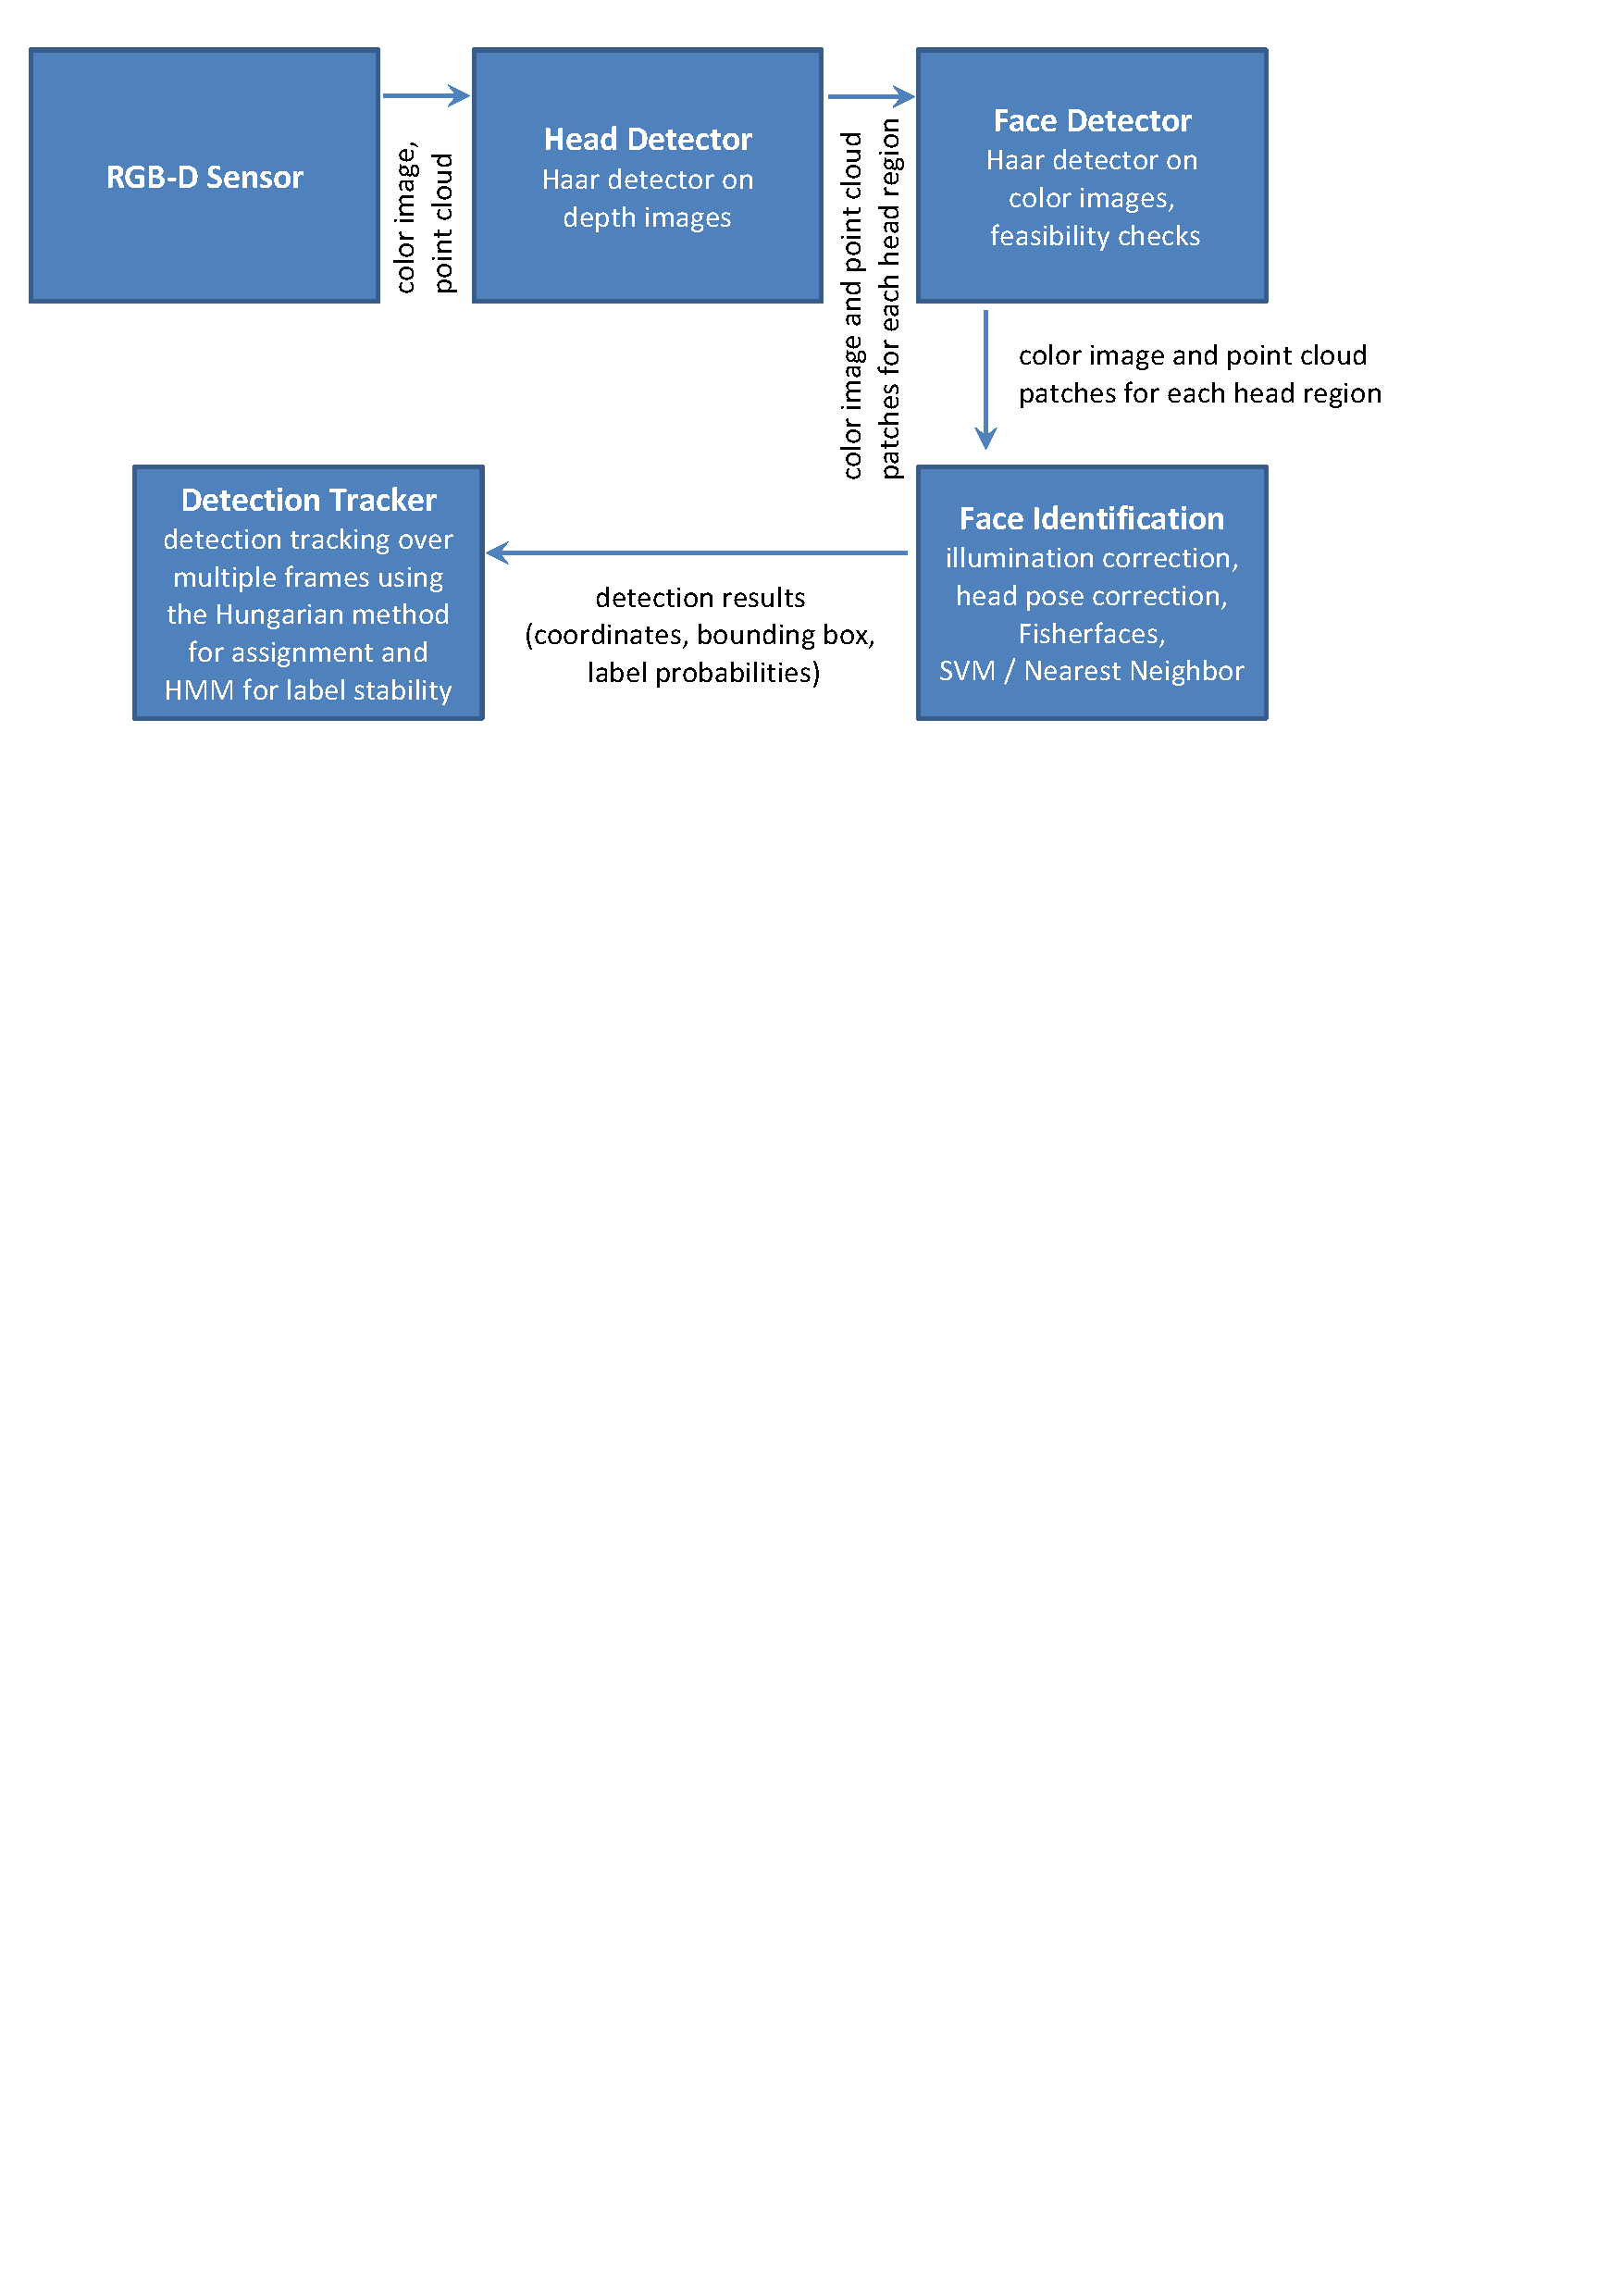
\includegraphics[width=0.99\columnwidth, trim = 4mm 280mm 40mm 4mm]{scheme2.pdf}
	\end{center}
	\caption{Computation scheme for the modules of the person recognition system with major algorithms outlined.}
	\label{fig:scheme}
\end{figure}

\section{RGB-D Face Detection}
\label{chap:methods:sec:detection}
%Algorithms for face recognition usually operate on image patches of face regions. Hence, the first step of the person recognition system is the detection of face regions in the image. 
To exploit the depth modality of the RGB-D sensor and to increase the detection performance, a head detection step in the depth image predates the actual detection of faces in the color image.
Both detection tasks are accomplished with the Viola-Jones detector \cite{Viola01}. %that scans the image with a sliding window and classifies image regions into face or no face based on boosted Haar features.
A well-trained classifier for color images comes already with the OpenCV library \cite{bradski2008} whereas the head classifier for depth images has been trained with own data from a Microsoft Kinect. 
For further details on the two-staged approach for face detection the reader is referred to our previous work \cite{Fischer2010}.
Additionally, we implemented further feasibility checks for the detected face regions. 
Face regions are only accepted up to a maximum distance $d_{max}$ to the camera which is mainly dependent on the resolution of the color camera and the corresponding expected accuracy at the face identification task.
Moreover, faces are only accepted if their 3d extent, i.e. the diameter of the head, lies within a realistic range $[h_{min}, h_{max}]$.

\section{RGB-D Face Identification}
\label{chap:methods:sec:identification}
The face identification approach assembles a variety of methods in three major steps to achieve robust recognition. \\
%The approach can be divided into three areas, where work has been done in order to achieve an overall improvement of the recognition framework.
\emph{Preprocessing:}
To mitigate the influences of uncontrolled real environments the images are preprocessed with respect to illumination and head alignment. 
%To overcome the issues of imagery, that is recorded in uncontrolled environments, the imagery is preprocessed regarding head pose and illumination of the scene.
This way more homogeneous input data for the actual recognition is produced. \\
	\emph{Recognition:} 
The normalized images are fed into a projection-based recognition system based on Fisherfaces. \\
%This recognition system involves an implementation of the Fisherfaces algorithm.
	\emph{Classification:}
Test images are projected to the subspace, that is computed during the training phase.
Traditionally the resulting feature vector is then compared to the projected training data and classification is done by choosing the nearest neighbor.
This framework also provides the possibility to classify the feature vector with machine learning methods such as Support Vector Machines or K-Nearest Neighbors.
%In order to be able to distinguish between people, that are already contained in the training data base and people new to it, a dynamically calculated threshold is used.

\subsection{Illumination Correction}
\label{chap:methods:subsec:illumination}
To compensate for illumination variation in uncontrolled lighting situations, a normalization to a standard form is performed.
We try to achieve uniform lighting conditions while retaining the facial features \cite{chen06}.
\subsubsection{Histogram Equalization}
The first processing step is a histogram equalization, which leads to a uniform distribution of
gray values throughout the image.
This becomes visible, as local contrast is increased \cite{Goel11}.
\todo{}
%- what is a histogram , what does it represent
%- why change the histogram
%- how change the histogram: formula, densitiy function maybe plot
%- results
%- drawbacks: only global illumination, spatial imbalance not considered

\subsubsection{Logarithm Transform}
In order to improve the illumination deficient, a logarithm transform can applied to the image
to expand low gray level and compress high gray level \cite{liu02}:
\begin{equation}
g(x,y)= \ln(f(x,y)+1) \quad .
\end{equation}
The original image is denoted as $f(x,y)$, the logarithm image is $g(x,y)$.
%- drawback: transform can overemphasize noise in  shadow areas..

\subsubsection{Gamma Transform}
\todo{}
%- illumination changes are in low frequency band of image - therefore trafo to freq domain
%- either truncating or scaling of low frequency coefficients - amplitude/influence is minimized
Another possibility is to apply a gamma correction, which avoids noise in dark areas of the image that can occur with the logarithm transform \cite{Tan2010}:
The gamma transformation can be calculated as:
\begin{equation}
	g(x,y)= f(x,y)^\gamma \label{eqn:gamma} \quad .
\end{equation}
The exponent $\gamma$ is the parameter the user can choose to control the strength of the transformation.

\subsubsection{Manipulation in frequency domain}
Following the rescaling of gray values, the image is transformed from a spatial representation to a frequency representation via a discrete cosine transformation (DCT):
The applied transformation is defined as:
\begin{equation}
  \begin{split}
    C(u,v)=\alpha(u)\alpha(v) \sum^{M-1}_{x=0}\sum^{N-1}_{y=0}g(x,y)\times \\ cos \left[ \frac{\pi(2x+1)u}{2M}\right]cos \left[ \frac{\pi(2y+1)v}{2N}\right].
  \end{split}
\end{equation}
The DCT coefficients are denoted as $C(u,v)$ and $u,v$ are coordinates in the coefficient block with the dimensions $M,N$.
The coordinates $x,y$ are pixel coordinates used in the spatial representation. 
Then, low-frequency coefficients are down-scaled as they contain illumination information \cite{Goel11}.
The number of scaled coefficients has to be balanced to minimize illumination variation 
but keep the discriminative power of facial features.
The overall illumination of the image can be controlled by the first DCT coefficient $C(0,0)$ \cite{liu02}.
Therefore it is set with respect to the desired average gray level $\mu$.
\begin{equation}
  C(0,0)= \log(\mu)*\sqrt{MN}
\end{equation}
Finally, the image is transformed back to the spatial domain via inverse DCT.
The next step is to reverse the transformation from the frequency representation to the spatial representation using the inverse DCT, which is defined as

\begin{equation}
  \begin{split}
    g(x,y)=\alpha(u)\alpha(v)C(u,v) \sum^{M-1}_{x=0}\sum^{N-1}_{y=0}\times \\ cos \left[ \frac{\pi(2x+1)u}{2M}\right]cos \left[ \frac{\pi(2y+1)v}{2N}\right].
  \end{split}
\end{equation}

%% equation: calculation of mu
This way of preprocessing effects that even disadvantageous illumination conditions can be compensated for.
The performance of this measure is evaluated in section \ref{ssec:EvalIllumination}.

\subsection{Head Pose Correction}
\label{chap:methods:subsec:pose}
A major drawback of appearance based recognition methods is the need for both the training data and 
the test data to be aligned as good as possible.
Deviation from pixel accurate alignment leads to degradation in recognition performance as is pointed out in \cite{Wagner2012}.
However, this can not be guaranteed in real world scenarios.
%As the subject is not constantly looking straight towards the camera the face image is subject to perspective distortions.
The automatic head pose correction aims at automatically aligning face images from their original recording perspective to a standardized virtual frontal recording perspective. % removing all effects of scale, translation and rotation.
This way, pose dependent intra class variation is minimized. % and higher recognition rates can be achieved in datasets with unaligned images.

%\begin{figure}[htbp]
%  \begin{center}
%    \def\svgwidth{0.8\columnwidth}
%    \includesvg{../images/CoordinateSystem}
%  \end{center}
%  \caption{Transformation from face coordinate system to world coordinate system}
%  \label{fig:FaceCoordinateSystem}
%\end{figure}

To establish the spatial relationship between the actual face orientation and 
 the normalized perspective, facial landmarks such as the position of the eyes and the nose are detected in the color image using the Viola-Jones detector \cite{Viola01}.
%The feature detection makes again use of the Viola and Jones object detector \cite{Viola01}. %, which was already used during the face detection stage \cite{Fischer2010}.
%Here it is applied for the detection of the left and right eye and the nose.
First, the nose is detected which enables a subdivision of the image into regions of interest for the left eye and the right eye.
This reduces both the number of ambiguous matches and the computation time. Then we determine the 3d coordinates of the facial landmarks from the depth image to construct the face coordinate system $X_{face}$: the $x$-axis points from the left to the right eye, the $y$-axis runs parallel to the nose and the $z$-axis is chosen orthogonally to the $x$ and $y$ axes in viewing direction. Next, we compute the transformation $T_{cam}$ that aligns the face coordinate system $X_{face}$ with the world coordinate system $X_W$ that is defined by the camera coordinate system of the RGB-D sensor. Transforming the recorded 3d face with $T_{cam}$ establishes a normalization w.r.t. rotation and translation. Finally, the 3d face is shifted in front of the camera with another transformation $T_{norm}$ and projected into a virtual image plane that captures the face frontally. Scale is normalized during the projection by choosing the camera matrix $K$ of the virtual camera in such a way that eyes and nose of the normalized 3d face are matched with a fixed face template. The whole transformation from the recorded 3d face coordinates $\mathbf{x}_{face}$ to the coordinates of the virtual frontal image $\mathbf{u}_{norm}$ is then:
\begin{equation}
  \mathbf{u}_{norm} = K T_{norm}T_{cam}\mathbf{x}_{face} \quad .
\end{equation}


We take advantage of the depth data, the RGB-D sensor provides by using the corresponding 
three dimensional coordinates of the facial landmarks.
The face coordinate system is defined according to Fig. \ref{fig:FaceCoordinateSystem} and the parameters of the three dimensional affine transformation $T_{norm}$ from the face coordinate system to the normalized perspective, are calculated.
To determine the head pose and the face orientation the face coordinate system $X_{face}$ is established.
The $x$-axis of $X_{face}$ is chosen in the direction of the eye base from the left eye to the right eye.
The coordinates of the detected nose are used to fix the $y$-axis. The $z$-axis is chosen orthogonally to the $x$ and $y$ axes in viewing direction.
This way differences in translation and rotation can be minimized.
The world coordinate system $X_W$ is the standard camera coordinate system of the Microsoft Kinect sensor according to Fig. \ref{fig:FaceCoordinateSystem}.
The world coordinate system $X_W$ is the standard camera coordinate system of the Microsoft Kinect sensor.
The coordinate system of the normalized perspective corresponds with the world coordinate system except for an offset in $Z$-direction.
By introducing a constant offset, the image scale is normalized.
By measuring the coordinates of the nose and the eyes, one obtains corresponding points in coordinate systems $X_{face}$ and $X_W$ and can therefore calculate the affine transformation $T_{cam}$.
The transformation to the coordinate system $X_{norm}$ of the normalized perspective remains as a simple translation in $Z$-direction.

The 3D data is transformed subsequently and projected on the virtual image plane, using the calibrated intrinsic camera parameters of the Kinect device in the camera matrix $C$.
\begin{equation}
  X_{norm}=C T_{norm}T_{cam}x_{face}
\end{equation}
The resulting perspectively normalized image corresponds to the virtual image taken from the normalized perspective.

\section{Face Recognition}
- general words
- image high dimensional feature vector
- division in training set and test images
\subsection{PCA}
\todo{}

The principal components analysis (PCA) uses an orthogonal projection $W$ to represent a set of possibly correlated variables with a set of linearly uncorrelated variables.

In this application PCA is used to generate a low dimensional set of features from a set of known images (training set).
The covariance matrix of the training set and its eigenvectors are calculated.
%- equation of covariance matrix
%- equation of eigenvalue problem
The $k$ eigenvectors with the biggest corresponding eigenvalues are used to form the orthogonal projection matrix $W$.
Thus every image of the training set can be represented by a linear combination of these eigenvectors.
%- equation of projection
The weights of this linear combination serve as feature vector for each particular image.

%- compression of image set is possible
%- for identification image is projected to
\subsection{Eigenfaces}
\todo{}
Eigenfaces is a popular projection based approach in face recognition, which applies PCA-based dimensionality reduction of involved images.
In the training phase of Eigenfaces, first the projection matrix $W$, which maximizes the global scatter of the training set, is computed with PCA.
Then each image of the training set is projected to feature space.
%- equation of the projection

In the recognition phase $W$ is used to determine the feature vector $x_test$ of a test image.
In feature space the distances between $x_test$ and the feature vectors of the training set can be calculated. 
These distances are called distances in face space (DIFS).

% - equation of DIFS
The recognition step is computationally very inexpensive and can therefore be used in realtime applications.
The method has been experimentally proven to work well under very controlled conditions, as it is very sensitive to variation of scale, illumination, expression.

\subsection{Fisherfaces}
\todo{}

Fisherfaces is a projection-based class specific based on Fisher's Linear Discriminant (FLD).
A linear projection $W$ is used to project the image from the high dimensional pixel-space to a feature space of much lower dimension.
In contrast to the Eigenfaces method, where principal component analysis (PCA) is used to maximize the total scatter among all images, Fisherfaces uses class information of the input data in the calculation of the projection and thus maximizes the inter-class scatter.
The projection directions of the optimal projection $W_{opt}$ are chosen orthogonal to intra-class scatter in order to overcome intra-class variation stemming from lighting changes or differing facial expression \cite{Belhumeur1997}.
As stated in literature, intra-class variations are often bigger than inter-class variation due to the recording conditions like illumination and head pose of the recorded subject \cite{Adini1997}.
Therefore it is crucial to recognition performance to maximize the inter class scatter.

The intra-class scatter matrix $S_W$ and the inter-class scatter matrix $S_B$ are calculated using the training set comprised of $C$ classes:
\begin{align}
  S_W&=\frac{1}{N_i}\sum\limits_{i=0}^{C}(m_i-m)(m_i-m)^T \\
  S_B&=\sum\limits_{i=0}^{C}\sum\limits_{j \in X_i}(x_j-m_i)(x_j-m_i)^T \quad .
\end{align}
Class $i$ contains $N_i$ images $x_j\in X_i$ whose mean is $m_i$. The mean image of the training set is indicated by $m$. % and $m_i$ the mean image of class $i$.
%The images of class $X_i$ are denoted as $x$.

%The projection $W_{opt}$ is calculated by applying Fisher's criterion.
%\begin{equation}
%  W_{opt}=\arg \max \frac{|W^T S_B W |}{|W^T S_W W|}
%\end{equation}
%In a face recognition application the intra-class scatter matrix is singular \cite{Belhumeur1997}.
To overcome the singularity of the intra-class scatter matrix, first, PCA is used to reduce the feature space to $N-C$ dimensions obtaining the PCA projection matrix $W_{PCA}$, followed by FLD to reduce the dimensionality to $C-1$. 
The final projection matrix $W_{opt}$ is defined as:
\begin{align}
  W_{PCA}&=\arg \max {\left|W^T S_T W \right|}\\
  W_{opt}&=\arg \max \left|\frac{W^T W^T_{PCA} S_B W^T_{PCA} W }{W^T W^T_{PCA} S_W W^T_{PCA} W }\right|  \\
  W_{opt}^T&=W_{FLD}^TW_{PCA}^T
\end{align}
%$W_{opt}$ contains generalized Eigenvectors.

\subsection{Classification and Identification of Unknown People}
\label{ssec:IdentificationUnknown}
%The resulting coefficients serve as feature vector and can be compared to the coefficients of the projected training images.
The projection $W_{opt}$ is used to project an arbitrary image $x$ to the feature space via $y=W_{opt} \cdot x$. 
%\begin{equation}
%  y=W_{opt} \cdot x  \quad .  \label{eqn:FisherProjection}
%\end{equation}
%This operation is performed for the images in the training set and for potential test images.
Classification is performed by finding out which classes's projected training data best describes vector $y$. %, obtained by projecting a test image into feature space.
Specifically, one searches for a sample $y_{i_k}$ of class $X_i$ which minimizes the Distance in Face Space (DIFS) to the projected test image $y_{test}$: %, which is calculated according to equation \ref{eqn:DIFS}
\begin{equation}
  \label{eqn:DIFS}
  DIFS=||y_{test}-y_{i_k}||^2
\end{equation}
Instead of calculating the Euclidean distance, the feature vector can also be classified by machine learning methods such as Support Vector Machines (SVM) or K-Nearest Neighbor (KNN).
The classification model has to be trained based on the training data before classification can be performed.

A typical application scenario for face recognition consists of people that are known to system $P_{k}$ and people that are unknown $P_{u}$.
In order to distinguish between those two groups during the classification step, a threshold in DIFS is introduced.
Whenever this threshold is exceeded, the test face is classified as part of $P_u$.
%An optimal selection of the values for this threshold is crucial to the recognition performance and for a practical application of the system.
The automatic threshold selection used here is based on information from the training data set only.
The maximal intra-class distance $D_{max,i}$ in feature space for each class serves as a measure of expansion of the projected images in feature space and hence their similarity.
The minimal inter-class distance $P_{min,i}$ gives an indication of the separation of the class clusters in feature space.
\begin{align}
  %\begin{split}
    D_{max,i} & =\max_{j,k \in X_i , j \neq k}\|W_{opt}(x_{j})-W_{opt}(x_{k})\|^2  \\
    P_{min,i} & =\min_{j \in X_i ,l \in X_m, m \neq i}\|W_{opt}(x_{j})-W_{opt}(x_{l})\|^2
  %\end{split}
\end{align}
The global threshold for the database is then defined as:
\begin{align}
  %\begin{split}
   \delta & = \min_{i=1,\ldots,C}\left(\frac{D_{max,i}+P_{min,i}}{2}\right)
   %\delta_i&=\frac{D_{max,i}+P_{min,i}}{2}
	%\end{split}
\end{align}
To allow for an effective selection of the threshold, a sufficient number of training images is required.

\subsection{Detection Tracking}
\label{sec:methods:subsec:tracking}

In robotic applications one usually has access to an RGB-D image stream. This provides the opportunity to connect and cross-check the detection results among multiple frames instead of analyzing each image in isolation. The goal of such a tracking of detections is to keep a history of identification results for each detected person to render the identification more robust and filter out sporadic false detections. %The algorithmic implementation of the tracking is twofold: first, the current detections are matched with detections from the previous image where applicable and second, the history of labels is updated and the most probable label becomes selected for each detected face.

The first task of matching previously detected faces with the current detections requires to define some measure of quality for a potential pair. With respect to (i) the high accuracy of the face identification on single images (ii) the high processing rate of the recognition system and (iii) the typical movement speed of persons and robots we assert the following matching costs between previous detection $i$ and current detection $j$:
\begin{align}
	c_{i,j} & = \left\| X_i - X_j \right\|_{L_2} + \left\| P_i - P_j \right\|_{L_2} \quad ,
\end{align}
where $X$ stands for the 3d coordinates of a detected face and $P$ denotes the probability distribution of each detection over all possible labels. Consequently, this costs function rewards if both detections appear at similar locations, which fits the assumptions of a high processing rate and a low movement speed of the persons, and if both detections have a similar prediction over the range of possible labels. The matching problem can be represented by a bipartite graph whose $N_p$ left-hand side nodes depict the set of previous detections and whose $N_c$ right-hand side nodes stand for the current detections. Both sets are fully connected with edges that carry the costs $c_{i,j}, i=1\ldots N_p, j=1\ldots N_c$. Finding the minimum costs matching in the weighted bipartite graph is known as the assignment problem. For solving this problem we apply the Hungarian method using the implementation of Rigdon \cite{rigdon2008_munkres}. New detections in the current image that have no matching previous detection are just added to the set of detections with their maximum likelihood label.

Having found the globally best fit of assignments we model the person identification process over time with a Hidden Markov Model (HMM) which naturally filters out singular false classifications. %Defining $l_t=q$ as the estimated label $q$ at time $t$, $o_t$ as the classifier's output label at $t$ and $\mathcal{L}$ as the set of possible labels the update rule is
%\begin{align}
%	p(l_t=q) & = \sum_{o_t\in \mathcal{L}}{p(l_t=q | o_t) p(o_t)}
%\end{align}
%where the HMM is defined as
%\begin{align}
%	& p(l_t=q | o_{t:1}) = \gamma \cdot p(o_t | l_t=q) \cdot \notag \\ & \sum_{q'\in \mathcal{L}}{p(l_t=q | l_{t-1}=q', o_{t-1}) p(l_{t-1}=q' | o_{t-1:1})}
%\end{align}
%with $\gamma$ being a normalization constant, $o_{t:1}$ representing the series of classifier outputs from time step $1$ to $t$ and the Markov property: $p(l_t=q | o_t) = p(l_t=q | o_{t:1})$. The classifier's prediction accuracy $p(o_t | l_t=q)$ is estimated from cross-validating the recorded data, the transition model $p(l_t=q | l_{t-1}=q', o_{t-1})$ simply assigns a high probability if both labels are equal, i.e. $q=q'$, and a low probability if they differ.
After updating the probability distributions over the available labels for the current detections, we finally need to decide for a unique label for each face. Considering the label probabilities as weights, this is again an assignment problem which is solved by the Hungarian algorithm. Should the label of a new face coincide with an already assigned label, the new detection is set back to the label 'Unknown'.

%- (rmb)
%- Hungarian method
%- Hidden Markov Models
%- clean double occurring labels (may occur )
%- proceed with tracking after short occlusions


\subsection{System Integration}
The person recognition system is fully implemented as a ROS package that can easily be downloaded and used. Standalone usage is facilitated with a simple control client provided with the package. The usage within a larger software project (C++ or Python) is similarly simple through the offered service interface that provides functions for automatic and manual image capture, training data access, classifier training, and recognition. Especially for users of Fraunhofer IPA's Care-O-bot the usage is fairly simple as the person recognition system is part of the Care-O-bot skill API.

%\subsubsection{Usage with Single Color Cameras}
%- maybe we add a paragraph how we adapted the algorithm to work with a single color only


%(rmb)
%- client protocol, services for data capture, classifier training, recognition
%- embedded in ROS framework
%- easy integration into larger scripts as a person identification skill (person detection as part of the Care-O-bot skill API)
%- user is capable of writing a simple state machine that queries unknown user for their name and captures some training images to recognize him the next time

      \cleardoublepage

      
\chapter{Evaluation}
\label{sec:evaluation}
The employed RGB-D face detection system has already been evaluated in \cite{Fischer2010} achieving a high recall rate of 98.0\% and a precision of 98.9\%. These results can be confirmed by an experiment described in Sec. \ref{sec:evaluation:subsec:headpose}.
%In previous work the face detection, that is part of the processing pipeline has been evaluated \cite{Fischer2010}.
However, this evaluation concentrates on verifying the performance of the face recognition system especially with respect to real world influences like varying illumination, head pose and facial expressions.
%To ensure its practicability it has been evaluated regarding influences, that can occur during its application in real world scenarios.
%Those influences include variations in illumination conditions, as the camera is not in a fixed position with controlled lighting but mounted on a mobile robot.
%The minimization of the influence that pose variation of the subject's head causes is also evaluated as well as varying facial expressions.
%Additional evaluation is done on the detection people, unknown to the database.
All experiments have been carried out on publicly available databases.
We tested Support Vector Machines (SVM), K-Nearest Neighbors (KNN) and Nearest Neighbor (NN) as classifiers.
As none of these methods proved to have a great advantage over another and for the sake of simplicity, NN based on Euclidean distance has been used throughout all experiments.
The parameters for the illumination compensation algorithms used in all experiments are $\gamma$-correction, which is set to $0.2$ \cite{Tan2010}, and the number of scaled DCT coefficients, which is 5 while the scaling factor is 50.

\subsection{Databases}
\subsubsection{Extended Yale Face Database B}
The Extended Yale Face Database B \cite{Georghiades01} comprises 38 subjects with 64 illumination conditions per subject.
%Some images are corrupted and are therefore excluded from testing.
All in all there are 2414 images used in the experiments.
These images were provided already cropped to a resolution of 192 x 168 pixels and display only a manually aligned face region of the subject in frontal perspective \cite{Lee05}.

\subsubsection{AT\&T database}
%Formerly known as Olivetti Research Ltd. (ORL) database  of faces \cite{Samaria1994}
The AT\&T database contains 10 images of 40 individuals in frontal pose, thus 400 face images in total.
The subjects were unrestricted in facial expression and the 4 female and 36 male were also allowed slight variations of pose.
%The subjects were unrestricted in facial expression so the 4 female and 36 male subjects can be depicted with open or closed eyes with or without glasses.
In contrast to the Extended Yale Face Database B facial outlines are visible and the images differ slightly in scale and alignment.
The images are manually cropped to a size of 92 x 112 pixels.
%\begin{figure}[t]
%	\begin{center}
%		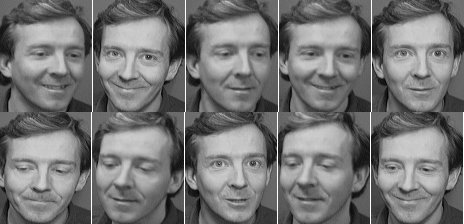
\includegraphics[width=0.9\columnwidth]{ATT_overview.jpg}
%	\end{center}
%  \caption{Typical subject from the AT\&T database of Faces.Sight slight variations in scale, pose and notable variations in facial expression are depicted}
%	\label{fig:att_overview}
%\end{figure}

\subsubsection{RGB-D Kinect Database}
The automatic head pose correction has been evaluated using data from the RGB-D Face Database \cite{Jasek2012}.
This database has been recorded using the Kinect sensor and contains color and depth data of 31 subjects recorded with 17 different head poses.
%There are 31 recorded people in 17 different head poses.
Each pose has been recorded 3 times, so altogether there are 1581 color and depth images.
To use the database for our purpose of solely analyzing the face recognition, face detection is applied beforehand and the face region in the depthmap and the color image is treated as input data for the evaluation.
%The use of the Microsoft Kinect sensor for the acquisition of this database makes it suitable for evaluation.

\subsection{Robustness to Illumination}
\label{ssec:EvalIllumination}
The implemented methods for illumination compensation have been evaluated on the extended Yale Face Database B.
According to \cite{Georghiades01}, the database was split into 5 subsets, with respect to azimuth and elevation of the light source direction with the camera axis as shown in Tab. \ref{YaleSubsets}.
\begin{table}[tb]
\caption{Subsets of the Extended Yale Face Database B}
\label{YaleSubsets}
\begin{center}
\begin{tabular}{c|c|c|c|c|c}
Subset & 1 & 2 & 3 & 4 & 5\\
\hline
Angle in [$^\circ$]  &0-10 & 10-25 & 25-50& 50-70 & $>$70\\
Number of Images & 263 & 456 &525 &456 &714\\ 
\end{tabular}
\end{center}
\end{table}
For the experiments, images with frontal and thus homogeneous illumination from  Subset 1 were used as training data.
Recognition tests were then carried out using subsets 2-5 as test data with an increasing difference in light source direction compared to the training data.
To make the impact of the illumination normalization step apparent, recognition results are reported for 
every test configuration with and without illumination compensation in Tab. \ref{tab:recognitionYale} and Fig. \ref{fig:illuminationcorrection} provides some examples of the preprocessing results.
For comprehensive comparison GammaDoG, a modified version of the illumination correction introduced by Tan et al. \cite{Tan2010} was also evaluated.
It is based on a gamma correction followed by filtering with a Difference of Gaussian filter and histogram equalization.
\begin{table}[htb]
\caption{Recognition rates on the subsets of the Yale database}
\label{tab:recognitionYale}
\begin{center}
\begin{tabular}{c|c|c|c|c}
Subset &  2 & 3 & 4 & 5 \\
\hline
%LBPH& 100\% &88\% &33.5\% &17.7\% \\
Eigenfaces& 95.83\% &51.43\% &12.06\% &3.081\% \\
Eigenfaces+LogDCT&100\% &84.38\% &70.175\% & 88.38\% \\ 
Fisherfaces& 100\% &94.0\% &39.70\%&5.74\%\\ 
Fisherfaces + HistEq &  100\% & 93.3\% & 62.7\% & 61.62\% \\ 
Fisherfaces + LogDCT & 100\% &94.3\% &85.7\% & 95.57\%\\
Fisherfaces + GammaDCT & 100\% &95.8\% &88.2\% & 96.2\%\\
Fisherfaces + GammaDoG & 100\% &99.4\% &98.0\% & 97.8\%\\
\hline
PP+LTP/DT \cite{Tan2010} & 100 \% & 100\% & 99.2 \% & 97.2 \% \\
\end{tabular}
\end{center}
\end{table}

\begin{figure}[t]
	\begin{center}
		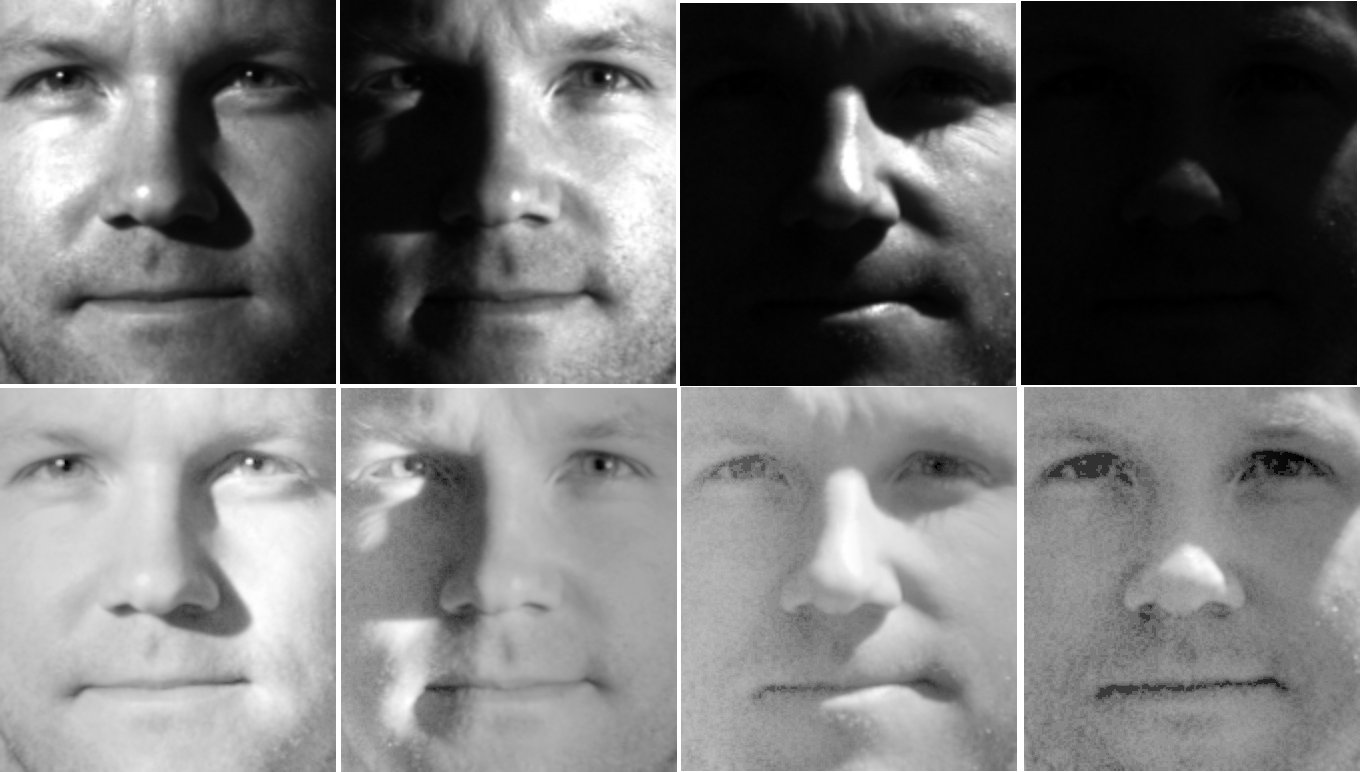
\includegraphics[width=0.9\columnwidth]{iluminationcorrection.jpg}
	\end{center}
	\caption{Illumination correction example (lower row) from Yale database. Images in upper row are taken from each subset from left to right with increasing angle between light source and camera view axis.}
	\label{fig:illuminationcorrection}
\end{figure}
As the angle of the light source increases, one can see a degradation of recognition rates of all tested algorithms, that do not include illumination compensation.
It is also apparent, that Fisherfaces handles illumination variation better than Eigenfaces, but its recognition rate is even further improved by including additional illumination normalization.  
Histogram Equalization improves recognition performance to some extent, but is outperformed by the other implemented methods.
The DCT coefficient scaling combined with a logarithm transform (LogDCT) and the DCT coefficient scaling combined with the gamma transform (GammaDCT) yield comparably good results, with a slight advantage for GammaDCT.
When Fisherfaces is combined with the GammaDoG illumination correction method the performance is furthermore improved.
Although staying slightly behind the top recognition rates of the state-of-the-art performance on the Yale Extended Database reported in \cite{Tan2010}, it is clearly shown that the improvement for Fisherfaces is significant when applying either GammaDCT, LogDCT or GammaDoG. Either of those methods can be chosen by a parameter in the provided software.
The results manifest a possible application of this recognition system in environments with lighting situations that are not covered by training data.


\subsection{Robustness to Facial Expressions}
The human face can express a variety of emotions. % among which are sadness, joy and anger.
Each one causes a notable distortion of the facial features, thus posing an additional
 challenge for the face recognition algorithm.
 To evaluate the stability of recognition performance with varying facial expression, the AT\&T database has been used.
 Tests to judge the performance under varying facial expressions included two testing strategies:
 \begin{enumerate}
   \item Leave-One-Out: 9 images per class were treated as training data and 1 image was used as test data.
   \item Leave-Half-Out: 5 images per class were treated as training data and 5 images were used as test data.
 \end{enumerate}
 Both testing strategies were carried out as tenfold cross-validation experiments, where training and test sets were chosen randomly.
 These evaluation protocols are proposed quite often in literature \cite{Naseem2010, Yang2002}.
 Recognition scores from literature are used for a comprehensive comparison of the proposed approach to state-of-the art techniques.
\begin{table}[htbp]
  \caption{Recognition rates on AT\&T database of faces}
	\label{table:att}
	\begin{center}
		\begin{tabular}{c|c|c}
		Subset & Leave-One-Out & Leave-Half-Out  \\
		\hline
		Fisherfaces& 98.75\% &95.9\% \\ 
		Fisherfaces +LogDCT& 95.8\% &94.4\% \\
		Fisherfaces +GammaDCT& 97.5\% &93.8\% \\
		Fisherfaces +GammaDoG& 87.5\% &93.8\% \\
		%FisherfacesOCV +GammaDCT&95.2\%\\ 92.9\%\\
		\hline
		LRC \cite{Naseem2010} & 98.75 \% & 93.5 \% \\
    ERE \cite{Wright2009} & 99.2 \% & 97.0 \% \\
		\end{tabular}
	\end{center}
\end{table}

The results obtained with Linear Regression (LRC) \cite{Naseem2010} are comparable to our results.
The best results are reported for Eigenface Regularization and Extraction (ERE), which achieve up to $3.2 \%$ better recognition rates than our implementation.
%The parameters of the preprocessing step were kept similar to the successful application in the examination of the performance under extreme lighting conditions.
Although all parameters of our method have been kept equal to the previous experiment a slight degradation of the recognition rates is apparent on this dataset with neutral lighting conditions for GammaDCT and to some extend for LogDCT compared to the pure Fisherfaces approach. Even more surprising, the GammaDoG normalization method causes a heavy drop in recognition rate on this database.
As GammaDCT yields more reliable results on datasets with neutral lighting and is only slightly worse under extreme conditions, it is chosen for the remaining experiments in this study.

\subsection{Robustness to Varying Head Pose}
\label{sec:evaluation:subsec:headpose}
The recognition experiments were carried out on image patches, where only the face of the person is visible.
Therefore all scenes in the database have been processed by the face detection algorithm described in section \ref{sec:methods:subsec:detection}. % after registering the color data to the depth data using the Kinect calibration data.
The face detection rates are documented in Tab. \ref{tab:EvalHeadPoseFaceDetection}, which also includes the detection rates reported by \cite{Jasek2012}.
The results are split up in results for the outer circle with viewing angles of ca. $50^\circ$ and the inner circle with about $30^\circ$ \cite{Jasek2012}.
One can see the detection rate dropping on the outer circle, but it is not influenced by varying facial expression.
It can be seen, that a $90\%$ of faces could be detected, without a single false detection.
As head pose normalization depends on finding facial features in the image, detection rates are also documented.
They are generally lower in poses on the outer circle but can cope with facial expressions very good.
\begin{table}[htbp]
  \centering
  \caption{Detection rates of faces and facial features on RGB-D DB}
  \label{tab:EvalHeadPoseFaceDetection}
  \begin{tabular}{p{2.0cm}|p{1.3cm}|p{1.3cm}|p{1.3cm}}
    pose & face detection rate& face feature detection rate & face detection rate \cite{Jasek2012}\\
    \hline
    All                  &  90.8 \%& 57.3 \%&51.7 \%\\
    Without outer circle &  95.7 \%& 66.3 \%&59.6 \%\\ 
    Only inner circle    &  95.4 \%& 63.1 \%&57.2 \%\\
    Only outer circle   &   75.3 \%& 26.1 \%&36.0 \%\\
    Facial expressions   &  95.7 \%& 95.4 \%&55.1 \%\\
    \end{tabular}
\end{table}

Images in which no face detection was possible have been excluded from the evaluation of the face recognition pipeline.
The retained cropped face images and depth maps have then been used to test the performance of the automatic head pose correction.
A cross-validation experiment has been conducted where half of the data from each subject is treated as training data and the other half as test data.
The recognition rate of $91.7\%$ is achieved on images, where faces could be detected successfully.
With respect to all images in the database $83.08\%$ of all images could be classified correctly.

In order to generate a very challenging test scenario regarding pose variation, dissimilarity in pose between training data and test data is simulated.
Therefore only images with a frontal head alignment were chosen as training images whereas the test data consisted of randomly chosen images, with variation in head pose.
10 classes have been randomly chosen, each of which provided 5 training images and 5 test images.
Please note that only images were considered, where face detection succeeded.
%The dissimilarity of the training set and the test set is documented in \ref{fig:EvalHeadPoseSetup}.
As the misalignment of faces is a major error source for the algorithm, it is tested if results can be improved by applying the automatic head pose correction described in Sec. \ref{sec:methods:pose}.
An improvement by applying both illumination normalization and head pose normalization is visible in Tab. \ref{tab:EvalPose} as well as in Fig. \ref{fig:headposecorrection}.
The overall recognition rates also indicate the difficulties for this algorithm in dealing with a big disparity of pose in training and test data.
\begin{table}
  \centering
  \caption{Recognition rates on dataset with big pose variation}
  \label{tab:EvalPose}
  \begin{tabular}{p{1.2cm}|p{1.2cm}|p{1.4cm}|p{1.4cm}}
    Method& no normalization &normalized illumination & normalized head pose \\
    \hline
    Eigenfaces & 36.2 \% & 52.7 \% & 61.8 \% \\
    Fisherfaces&41.5 \% & 56.3 \% & 68.1\% \\
  \end{tabular}
\end{table}
%\begin{figure}[htbp]
%  \begin{center}
%    \def\svgwidth{0.8\columnwidth}
%    \includesvg{../images/test}
%  \end{center}
%  \caption{\todo{describe}}
%  \label{fig:EvalHeadPoseResults}
%\end{figure}

%Results
\begin{figure}[t]
	\begin{center}
		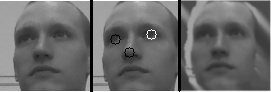
\includegraphics[width=0.9\columnwidth]{headposecorrection.jpg}
	\end{center}
	\caption{Example for the head pose correction.}
	\label{fig:headposecorrection}
\end{figure}
%discussion and interpretation

\subsection{Results in Real World Situations}
Besides the great results on common database tests we also like to emphasize the suitability of the proposed framework in real situations. To show the applicability in real applications we recorded a dozen of real situations in which some of 8 people from our lab were present. The scenes contain people working in their office, sitting at a dining table and a sofa, and show hard cases when illumination, head pose and facial expression vary. A nice overview over these scenes can be gained from the accompanying video. Fig. \ref{fig:covergirl} also displays one of those scenes. All 8 persons have been trained in all of the videos. The video also demonstrates the real time applicability of our system, which needs 250~ms for the detection step, 80~ms for head pose correction and 8~ms for the recognition with illumination normalization on a single core of a i7 2600K, 3.4 GHz.

%Record some data sets (ca. 10) with the following free parameters:
%- ground truth faces learned only in one single situation with certain conditions (conditions may be different for different people)
%- numerous people (ca. 10)
%- different head orientations
%- light switched on/off
%- indoor/outdoor
%- facial expressions
%- moving people
%- realistic situations (i.e. cob lab: kitchen, sofa, table, ...)
%- unknown people
%
%Success is judged on the accumulated tracking results, i.e. have the people been labeled correctly most of the time.
%
%- runtime (rec+illum: 8ms,  rec+illum+head: 80ms, face det. 250ms) single core i7 2600K, 3.4 GHz, 16 GB RAM

\subsection{Recognizing Unknown People}
In order to judge the practicability of the threshold selection mentioned described in Sec. \ref{ssec:IdentificationUnknown}, the recognition performance on two databases was examined regarding classification.
For the experiment, the database was divided into two subsets. Half of the classes were not included in the training data, thus keeping the excluded people unknown.
Of the remaining subset, half of the images of each class was used as training data.
The test data consists consequently of images of both unknown and known individuals.
This experiment was carried out on the Extended Yale Database B and the AT\&T database.
The division into subsets is done according to table \ref{tab:EvalUnknownDivision}.

\begin{table}[htbp]
  \centering
  \caption{Subdivision of databases that were used for evaluation identification of unknown people}
  \label{tab:EvalUnknownDivision}
  \begin{tabular}{c|p{0.8cm}|p{0.8cm}|p{0.8cm}|p{0.8cm}|p{0.8cm}|p{0.8cm}}
    Database&\multicolumn{3}{|c|}{Training Set}&\multicolumn{3}{|c}{Test Set}\\
    \hline
    &images & classes known & classes unknown& images & samples known & samples unknown\\
    \hline
    AT\&T &100 & 20 &20 & 300 & 100 & 200\\
    Yale & 605 & 19 &21 & 1809 & 603 &1206\\
  \end{tabular}
\end{table}

The classification is only considered correct when either an unknown person is classified unknown, or a known person is assigned to the right class.
Training data and test data was chosen randomly and recognition rates were verified using tenfold cross-validation.
Results can be seen in Tab. \ref{tab:EvalUnknownThreshold}.

%\begin{figure}[htbp]
%  \begin{center}
%    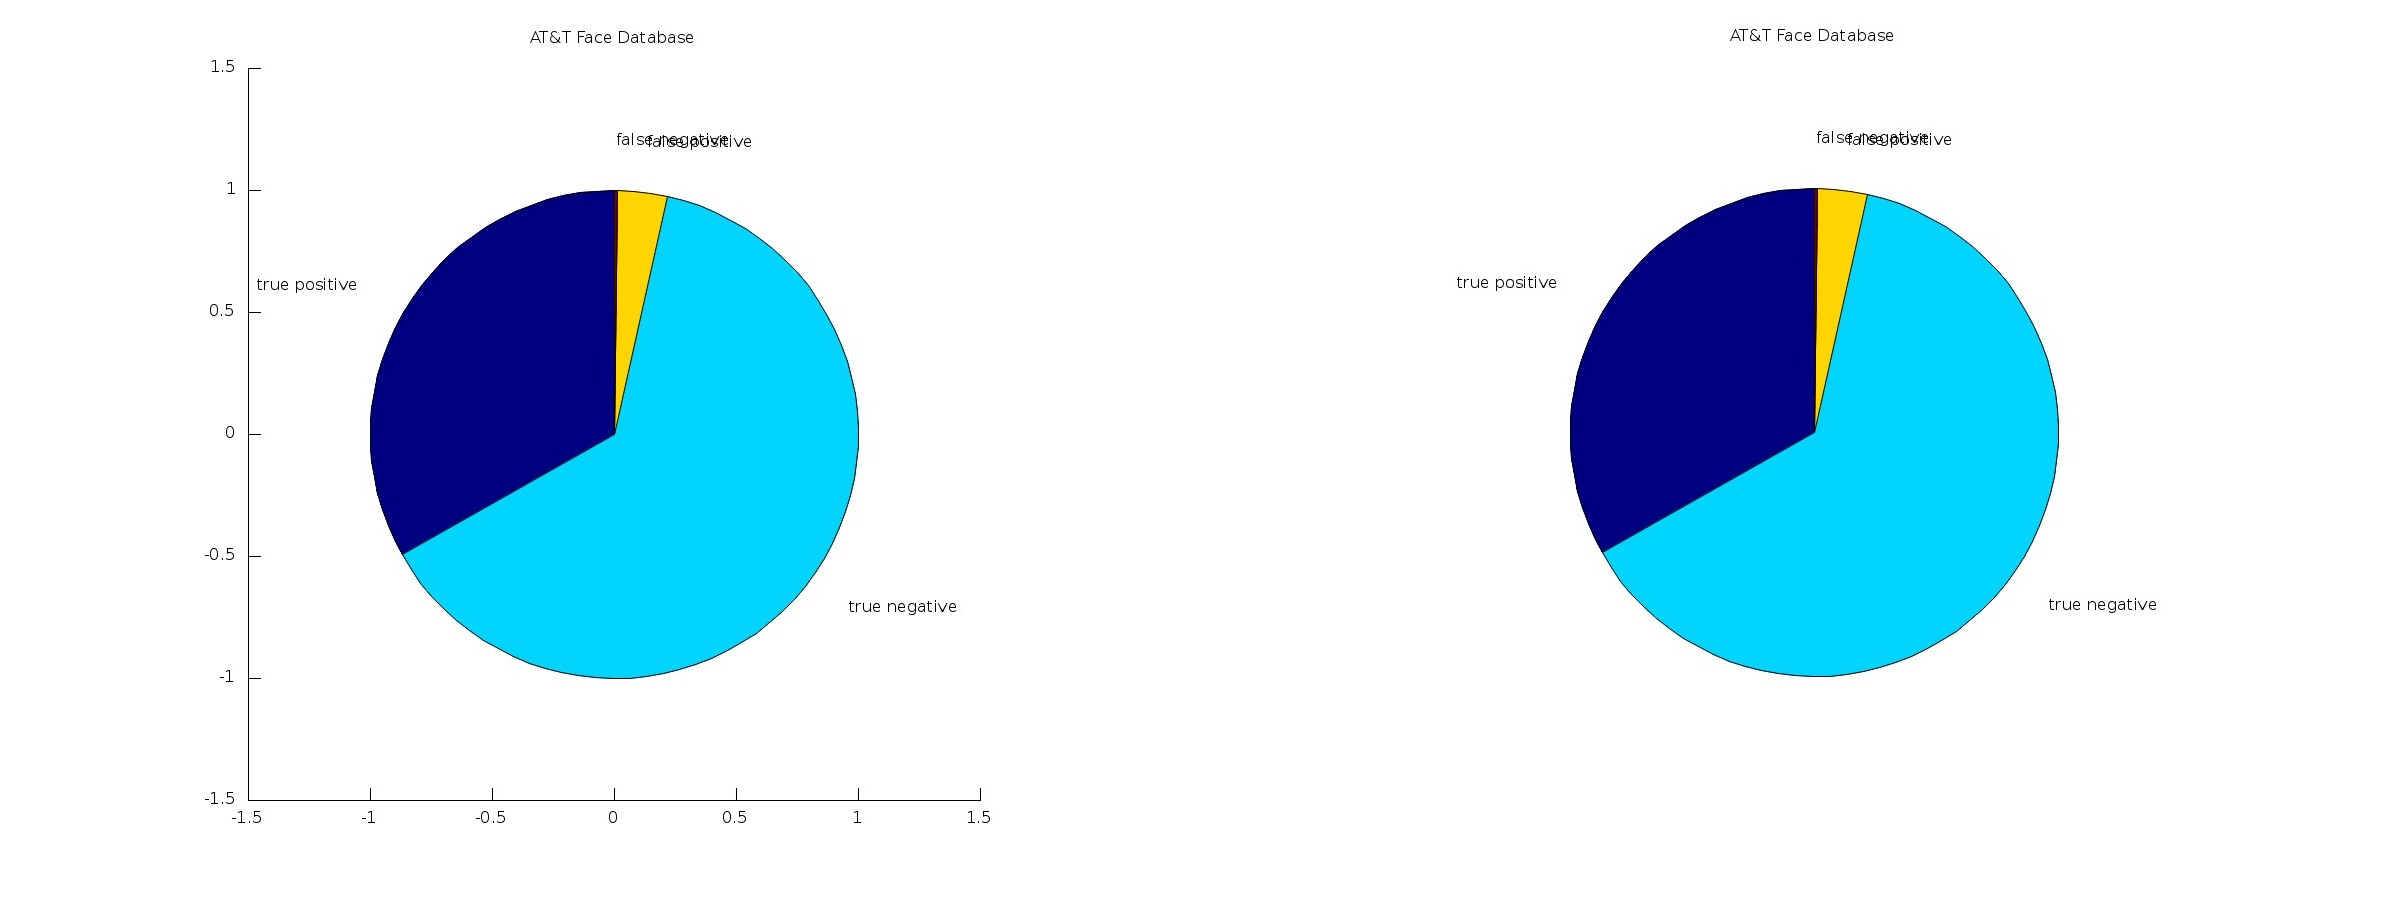
\includegraphics[width=0.8\columnwidth]{PieUnknownATTYALE.jpg}
%  \end{center}
%  \caption{\todo{describe+minipage + table + intuitive colors in grayscale}}
%  \label{fig:EvalUnknownPie}
%\end{figure}

\begin{table}[htbp]
  \centering
  \caption{Results for recognition of unknown people}
  \label{tab:EvalUnknownThreshold}
  \begin{tabular}{l|p{0.8cm}|p{0.8cm}|p{0.8cm}|p{0.8cm}|p{0.9cm}}
    Scenario & True \newline Positive & False \newline Positive & False \newline Negative & True \newline Negative  &   Recognition rate\\
    \hline
    AT\&T &82.4 \%  & 17.6\% & 2.4\% & 97.6\%& 92.5 \% \\
    Yale & 99.4 \%& 0.5 \%& 4.93\% & 94.9\% & 96.5 \% \\
  \end{tabular}
\end{table}
The results on the tested databases show, that the dynamic threshold application has the potential of distinguishing between known people and unknown people.
Although the size of the training data sets is different for both databases, our solution still achieves a high overall recognition rate of over $90 \%$ in both cases.

%\subsection{Single Color Camera}

      \cleardoublepage

      
\section{Conclusions and Outlook}
\label{sec:conclusions}
In this paper we presented a comprehensive framework for the detection and identification of people. The software utilizes a couple of novel and state-of-the-art methods and achieves compelling results for face detection as well as for face recognition tasks. Even under heavy conditions like varying lighting the system could consistently obtain recognition rates over 90\%. The robustness against head pose and facial expressions on standard database tests as well as in real life operation was convincing. The recognition system's computational demands are low enough for the application on mobile service robots. The availability of the whole software as free and open-source is intented to help other developers to faster implement complex robotics applications that depend on user.

%- wrap up the main outcomes of the paper

Future work aims at the implementation of automatic capturing of additional training images of known persons during operation in situations when the current configuration fails or has a small margin to other identifications. Furthermore, the integration of whole body detection and tracking for person detection is planned to enable model-based tracking beyond the current face or head tracking. Finally, we envisage to analyze the potential additional benefits of using the depth images also for identification as proposed in \cite{Tsalakanidou03}.

      \cleardoublepage
      %% TEMP

      %%\newpage
\section{Recognition}


 General definition of face recognition as classification task.

 Different kind of approaches.

Appearance based approaches used in this work.

Definition of image space.
Definition of feature space.

Calculations in \textit{image space} are computationally expensive and  therefore
one applies dimensionality reduction to a \textit{feature space}.

Requirements for feature space:
\begin{itemize}
\item Reduced dimensionality for lower computation cost
\item Optimized for classification task - no smearing but clustering of samples of indicidual classes
\end{itemize}

In this work two approaches are used: Eigenfaces, Fisherfaces.
Both consist of a two phase structure:

Training phase for construction of feature space.

Recognition phase for classification of samples.


\subsection{Training phase}
Set of training images ${ x_j }$, which consists of $N$ images is used to train a model.
The set is divided in classes, which in case of face recognition and classification are
 different people. The number of classes in the training set is denoted as $c$.

\subsection{Recognition phase}
Previosly trained model is used to project the recognition sample to the feature space.
Classification methods used to find class, sample belongs to.


\section{Principal Component Analysis (PCA)}
Principal component analysis is common method in computer vision for dimensionality reduction.
Linear transformation from image space to feature space.

Dimension reduction based on total Scatter of training set.
Dimensions: From n(image size) to m.


Computation of mean image $m$.
\begin{equation}
m=\frac{1}{N}\sum\limits_{j=0}^{N-1}{x_j}
\end{equation}

Computation of total scatter matrix.
Explanation of scatter matrix/correlation matrix.

\begin{equation}
S_T=\frac{1}{N}\sum\limits_{j=0}^{N-1}(x_j-m)(x_j-m)^T
\end{equation}

Calculation of the linear projection.Aim is to maximize the determinant
 of the total scatter matrix.
\begin{equation}
W_{PCA}=\arg \max |W^T S_T W |
\end{equation}
Eigenvalue decomposition results in the projection matrix $W_{PCA}$.

Projection matrix consists of Eigenvectors corresponing to the $m$
largest eigenvalues from the decomposition.


\section{Linear Discriminant Analysis (LDA)}
Dimensionality reduction based on linear projection.
Between-class scatter is maximized opposed to within-class scatter.
Dimensions: From n(image size) to m (number of classes -1).


The within-class scatter matrix $S_W$ and the between-class scatter matrix $S_B$ are calculated:
\begin{equation}
  S_W=\frac{1}{N_i}\sum\limits_{i=0}^{c}(m_i-m)(m_i-m)^T
\end{equation}

\begin{equation}
  S_B=\sum\limits_{i=0}^{c}\sum\limits_{j \in X_i}(x_j-m_i)(x_j-m_i)^T
\end{equation}

Where $N_i$ are are the number of images per individual class, $m_i$ denotes the mean image of
each class.


\begin{equation}
  W_{LDA}=\arg \max \frac{|W^T S_B W |}{|W^T S_W W|}
\end{equation}
Solved by generalized eigenvalue problem. $W_{LDA}$ consists of Eigenvectors, corresponding
to the m biggest Eigenvalues.
Attention, when  $S_W$ is singular.(As is the case without PCA).

\section{Eigenfaces}
A linear transformation is computed, that maps the $n$-dimensional \textit{image space} to
the $m$-dimensional \textit{Eigenspace}.
So the image is transformed to a feature vector $y_k  \in \mathbb{R}^m$.

\begin{align}
  W_{opt}& =W_{PCA}\\
  y_k    & =W_{opt}^T x_k \\
\end{align}

\subsection{procedure}
Perform dimension reduction with PCA of training set.

Result is projection matrix $W_{PCA}$.

Probe images are projected to subspace by applying $W_{PCA}$.

Performance depends on dimension of subspace - number of eigenvectors.

Nearest neighbour based classification of sample is performed in subspace(Eigenspace).

\subsection{drawbacks - improvements}
Eigenfaces are sensitive to illumination changes.

Performance of approach dependent on dimension of feature space.

Only total scatter is considered , the information of classes in the training set is
neglected. Within-class scatter is treated in the same way as between-class scatter.
Method not optimized for clustering/classification in feauture space - one needs
method, that is optimized for classification.


Solution:

Proposal of eliminating first three principal comonents - mainly influenced from lighting.
But one also loses discriminative information in the components.

Use of additional optimization of feature space with respect to different classes.

\section{Fisherfaces}
 Class-specific method, that takes advantage of the labeled training set.

Within-class scatter is distinguished from between-class scatter. 

Problem within-class scatter matrix is most likely singular.

LDA criterion is extended to match the application in face rcognition.


\begin{align}
  W_{opt}& = W^T_{LDA}W_{PCA}\\
  W_{PCA}& =\arg \max |W^T S_T W |\\
  W_{LDA}& =\arg \max \frac{|W^T W^T_{PCA} S_B W_{PCA}W |}{|W^T W^T_{PCA} S_W W_{PCA} W|}
\end{align}

PCA throws away only the smallest principal components, which contain the less discriminative information
compared to the largest principal components.

\subsection{procedure}
Dimension reduction is first performed by PCA ( from $n$) to $N-c$.

Training set is projected to PCA subspace by applying $W_{PCA}$.

LDA is then applied, in order to achieve a subspace, that enables classification.

The dimension of the final subspace is $c-1$.

      %%\section{FaceNormalizer}
Class is designed to account for change in recording perspective and illumination conditions.
It can be used in both the acquisition of training data and the actual face recognition process.

Flowchart \ref{fc:FaceNorm} depicts the workflow, that is contained within the class FaceNormalizer.
An detailed explanation of the single functions is given below.


\begin{figure}
\centering
\inputTikZ{../tikz/fc-FaceNorm}
\caption{Overview of face normalization process.}
\label{fc:FaceNorm}
\end{figure}

\subsection{Radiometric Normalization}

In order to limit the influence of varying lighting conditions a radiometric normalization is 
applied to each input image as a preprocessing step.
To enhance the radiometry of the input image, the algorithm as depicted in figure \ref{fc:RadNorm}
and described below is applied.
It can be used on both $RGB/BGR$ and grayscale images.

\begin{figure}
\centering
\inputTikZ{../tikz/fc-RadNorm}
\caption{Flowchart of radiometric normalization.}
\label{fc:RadNorm}
\end{figure}

In the following, the single steps of this lighitng correction are described. For grayscale input images
only steps $4-7$ are needed.
\begin{enumerate}
\item Transformation from RGB/BGR colorspace to HSV colorspace
\item Extraction of the value channel(V),furhter processing takes place on single channel
\item Transformation to logarithmic domain
\item Discret Cosine Transformation(DCT)
\item Coefficients of DCT are truncated in order to filter out low frequencies
\item Inverse DCT (IDCT), to reverse transformation
\item Exponential transformation to reverse logarithmic transform
\item Merging of the original hue and saturation channels with the equalized value channel
\item Transformation back to RGB/BGR colorspace
\end{enumerate}

\subsection{Size Normalization}
Depending on the distance to the camera, a face object conatained in a image region of varying size.
In order to have comparable data for recognition, all input images are resized to the same dimension.
Therefore a interpolation method \textit{bilateral interpolation} is selected.

\subsection{Geometric Normalization}

\begin{figure}
\centering
\inputTikZ{../tikz/fc-GeomNorm}
\caption{Flowchart of geometric normalization.}
\label{fc:GeomNorm}
\end{figure}

During the capturing process of input images, the pose of the head is not controlled.
Therefore one has to consider changing alignment of the facial features in input images.
In order to reduce this crucial error, geometrical alignment is applied to each input image.
\begin{enumerate}
\item Facial feature detection
  \begin{enumerate}
  \item Detection of the nose and subsequent division of input image into search regions 
        for other facial features.
  \item Detection of eyes and mouth.
  \end{enumerate}
\item Calculation of target positions of nose and mouth, based on image proportion, derived
      from image measurements.
\item -------- without available depth information
\item Calculation of affine transformation, where the detected facial features serve as homologue
      points.
\item Affine transformation is applied to image(\textit{image warping}).
\item -------- wen depth information is available
\item Calculation of perspective transformation, using 3D information, when available
\item Application of perspective transformation on 3D Pointcloud, with attached RGB values
\item Filtering of output to enhance image quality

\end{enumerate}
\begin{figure}[h!tbp]
\centering
  \def\svgwidth{=0.8\textwidth }
  \includesvg{../img/GeomFaceNorm}
\caption[Detection of facial features]{The sketch on the left depicts an unnormalized input image. The red crosses
        represent the detection of eyes,nose and mouth. The dashed lines separate the original image into search regions
        for the particular features.The distances $a,b,c$ represent the distances between the detections. The right sketch
        depicts the norm face with corresponding norm distances $A,B,C$. Of those only $A$ is defined a priori. $B,C$ are
        calculated according to equations \ref{ss:NormDist}}.
\label{fig:FeatDet}
\end{figure}

\subsubsection{Derivation of norm distances $A,B,C$}
\label{ss:NormDist}
One intends to keep the original proportions of the specific face.
Therefore only the distance between the two eyes $A$ is fixed a priori. Distances $B,C$ are determined by equation
 \ref{eqn:NormDist}.
\begin{align}
\label{eqn:NormDist}
B&=\frac{A}{a/b}\\
C&=\frac{A}{b/c}
\end{align}

The distances determine the $Y$-coordinate of mouth and nose according to equations.
The $X$-coordinate of the norm features is based on the assumption of a symmetric face.

\begin{align}
X_{mouth}&=X_{lefteye}+0.5A\\
Y_{mouth}&=Y_{lefteye}+C\\
Y_{nose} &=Y_{lefteye}+B\\
\end{align}


For the case, when not enough facial features can be detected, the warping process is skipped.
During the acqusisition of training data, images are processed until one normalization is completed
succesfully. In contrast to that, during recognition the radiometrically and sizewise normalized image is passed on
to the recognition stage even without the pose compensation.


\subsubsection{Example}
\begin{figure}[h!tbp]
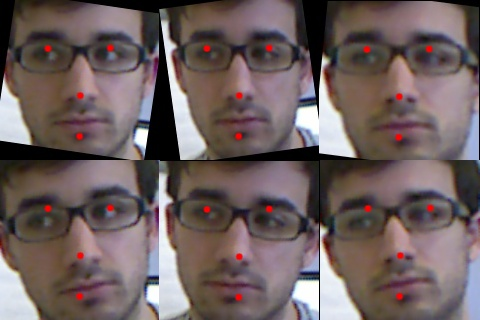
\includegraphics[width=1.0\textwidth]{../img/norm_geometric.jpg}
\caption{This figure depicts a set of three images, that have been processed by the geometrical normalization
algorithm. The artificially added red dots show the norm positions of eyes, nose and mouth.}
\label{fig:NormFace}
\end{figure}
Figure \ref{fig:NormFace} shows that by the geometrical normalization the misalignment of faces due to a varying head pose 
can be overcome or at least minimized.


\subsection{Geometric normalization with depth information}
When there is depth information available for the face image, one is able to use this information for the warping transformation.

\begin{itemize}
\item Get points in point cloud, that correspond to the detected face features
\item Calculate the pose and position of a virtual camera with respect to the 3D points and the norm previos
ly determined norm coordinates of the face features.
\item Resample the pointcloud (RGBXYZ) from the calculated pnp
\item Filter resulting image to compensate for occlusions and poorly sampled pointcloud in image regions
\end{itemize}




\listoftables
\listoffigures


\bibliographystyle{plain}
\bibliography{../../literature/DA_literature}
\end{document}

